\documentclass{paper}

%\usepackage{times}
\usepackage{epsfig}
\usepackage{graphicx}
\usepackage{amsmath}
\usepackage{amssymb}
\usepackage{color}
\usepackage{caption}
\usepackage{subcaption}

% load package with ``framed'' and ``numbered'' option.
%\usepackage[framed,numbered,autolinebreaks,useliterate]{mcode}

% something NOT relevant to the usage of the package.
\setlength{\parindent}{0pt}
\setlength{\parskip}{18pt}






\usepackage[latin1]{inputenc} 
\usepackage[T1]{fontenc} 

\usepackage{listings} 
\lstset{% 
   language=Matlab, 
   basicstyle=\small\ttfamily, 
} 



\title{Report for assignment 1}



\author{Moser Stefan\\09-277-013}
% //////////////////////////////////////////////////


\begin{document}



\maketitle


% Add figures:
%\begin{figure}[t]
%%\begin{center}
%\quad\quad   \includegraphics[width=1\linewidth]{ass2}
%%\end{center}
%
%\label{fig:performance}
%\end{figure}

\section{Photometric Stereo (Due on 29/10/2013)}

\subsection{Calibration}
In this chapter I describe, how the light directions can be retrieved by 
inspecting the specular reflection of a sphere.

\subsubsection{Calculating the light direction} 
We know, that every point on the sphere must satisfy
\begin{equation}
	r^2 = x^2 + y^2 + z^2
\label{eq:sphere_coord}
\end{equation}
for the cartesian representation of a sphere as $(x,y,z)^T$ with the radius $r$. We can deploy this constraint, by bringing the bright
 highlight into the sphere coordinate system. This is simply done 
 by subtracting the center of the sphere. The variables used in eq. \ref{eq:light_direction} are:
\begin{itemize}
\item The 2D coordinates of the light source $i$'s highlight on the sphere, named $p_i$. It is computed as centroid of all points above a certain brightness threshold
\item The 2D coordinates of the centre of the sphere $c$, computed as the centroid of the mask.
\end{itemize}
\begin{equation}
	n_i = 
	\left[ 
	\begin{array}{c}
	(p_i - c)_x \\
	(p_i - c)_y \\
	-\sqrt{r^2 - (p_i - c)_x^2 - (p_i - c)_y^2}
\end{array} 
\right] 
\label{eq:light_direction}
\end{equation}
For the z coordinate, eq. \ref{eq:sphere_coord} can be solved for z. The negative solution is the correct choice, since it is the one pointing towards the camera.

Once the normal at the lights highlight are retrieved, they can be used with ray reflection to get the direction towards the light
\begin{equation}
	L_i = d - 2(d\cdot \hat{n}_i)\hat{n}_i
\end{equation}
with $\hat{n}_i$ being the normalized vector of $n_i$ and $d$ the direction of a light ray from the camera towards the sphere.
The assumption given in the assignment is, 
that every ray originating from the camera has direction $d = (0,0,1)$ for every point of the image.

\subsubsection{Results}
All light directions $L_i$ can be assembled into a matrix $\mathbf{L}$. Here the
transposed version is shown, since it is easier to fit on a page.
\begin{align*}
\mathbf{L}^T= 
\left[ 
\begin{array}{cccccccccccccc}
0.4507 & -0.4230 & -0.7861 \\ 0.2180 & -0.1229 & -0.9682 \\ -0.0345 & -0.1577 & -0.9869 \\ -0.0854 & -0.3983 & -0.9133 \\ -0.2897 & -0.4593 & -0.8397 \\ -0.1012 & -0.5080 & -0.8554 \\ 0.2540 & -0.3823 & -0.8885 \\ 0.0908 & -0.3885 & -0.9170 \\ 0.1856 & -0.3014 & -0.9353 \\ 0.0794 & -0.2990 & -0.9510 \\ 0.1158 & -0.0415 & -0.9924 \\ -0.1295 & -0.3261 & -0.9364 
\end{array} 
\right] 
\end{align*}
They are fairly close to the defaults given. The mean squared error over all normalized directions is 0.0217.

\subsection{Computing Surface Normals and Grey Albedo}

\subsubsection{Calculations}

For computing the grayscale albedo, I first reduced the color information to a single channel by computing the luminance $\ell$
\begin{equation}
	\ell = c_\text{red} \cdot 0.299 + 
		c_\text{green} \cdot 0.587 + 
		c_\text{blue} \cdot 0.114
\end{equation}
for each image. 

In the lecture it was shown, that we can compute the normals by solving
\begin{align*}
	 I &= S\tilde{n} \\
	 S^TI &= S^T\tilde{n} \\
	 \tilde{n} &= (S^TS)^{-1}S^TI
\end{align*}
with 
\begin{itemize}
	\item $I$ a vector of the luminance values of the 
	inspected pixel for all $n$ images
	\item $S$ a matrix of all light directions, with each row
	having the light direction of the corresponding image.
	\item $\tilde{n}$ the normal direction (not unit size)
	
\end{itemize}
Further, we know that we can obtain the grayscale albedo $\rho$ by taking the length of $\tilde{n}$
\begin{equation}
	n = \frac{\tilde{n}}{\rho}
\end{equation}
Once we know the normals, we can use them to compute the color albedo $a$, using
\begin{align*}
	I &= a(n \cdot L) \\
	(n \cdot L)^{-1} I &= a
\end{align*}
on every pixel.

\subsubsection{Results}
\begin{figure}[h!]
        \centering
        \begin{subfigure}{0.3\textwidth}
                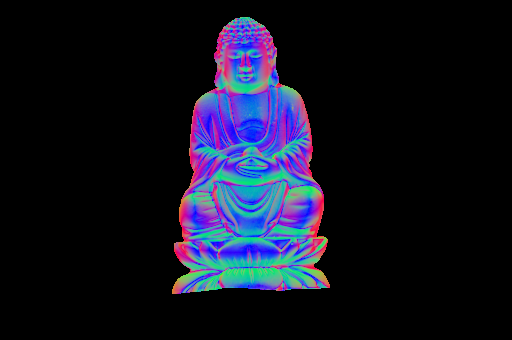
\includegraphics[width=\textwidth]{report_fig/buddha_n}
        \end{subfigure}
        ~ 
        \begin{subfigure}{0.3\textwidth}
                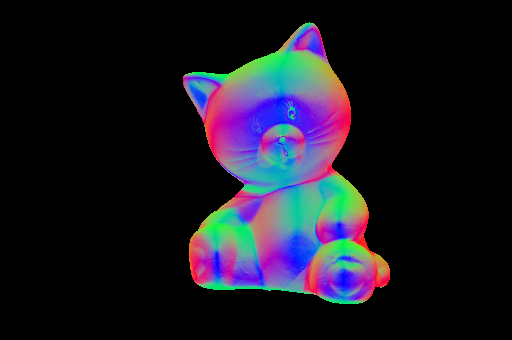
\includegraphics[width=\textwidth]{report_fig/cat_n}
        \end{subfigure}
        ~ 
        \begin{subfigure}{0.3\textwidth}
                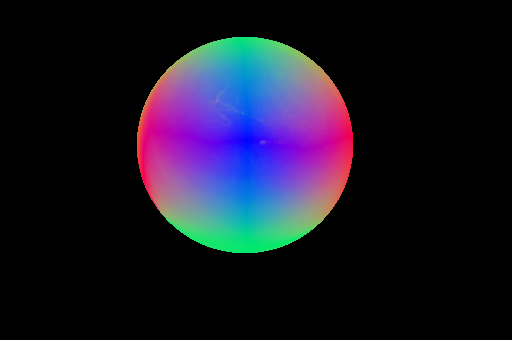
\includegraphics[width=\textwidth]{report_fig/gray_n}
        \end{subfigure}
        % second row
        \begin{subfigure}{0.3\textwidth}
                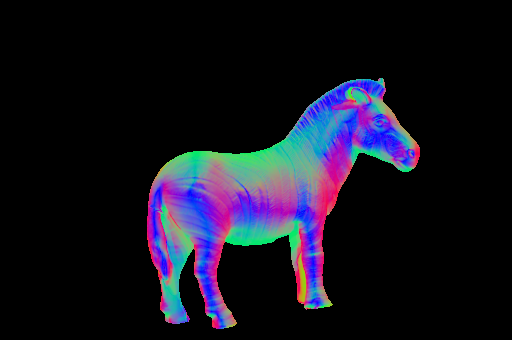
\includegraphics[width=\textwidth]{report_fig/horse_n}
        \end{subfigure}
        ~ 
        \begin{subfigure}{0.3\textwidth}
                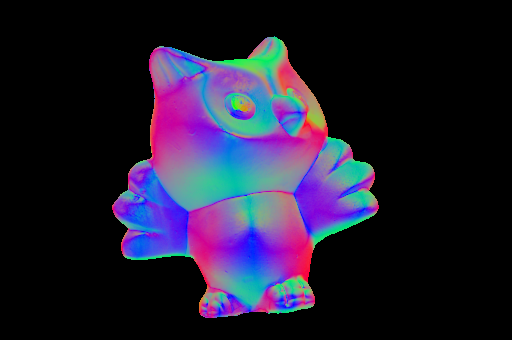
\includegraphics[width=\textwidth]{report_fig/owl_n}
        \end{subfigure}
        ~ 
        \begin{subfigure}{0.3\textwidth}
                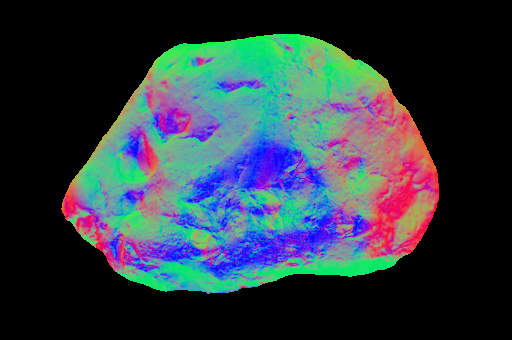
\includegraphics[width=\textwidth]{report_fig/rock_n}
        \end{subfigure}
        \caption{The normals visualized for every scene. For transforming
         them into rgb range, I took the absolute value. The background 
         (where the mask is zero) is shown black. }
        \label{fig:normals}
\end{figure}
\begin{figure}[h!]
        \centering
        \begin{subfigure}{0.3\textwidth}
                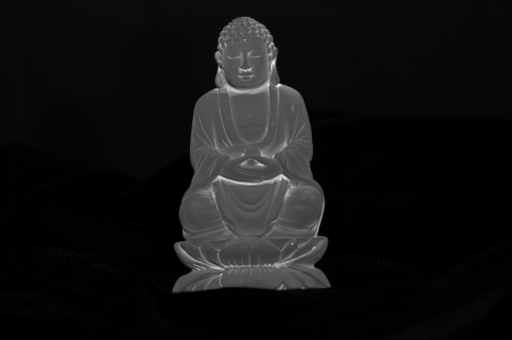
\includegraphics[width=\textwidth]{report_fig/buddha_a}
        \end{subfigure}
        ~ 
        \begin{subfigure}{0.3\textwidth}
                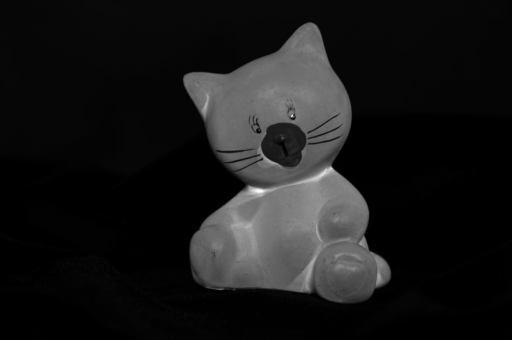
\includegraphics[width=\textwidth]{report_fig/cat_a}
        \end{subfigure}
        ~ 
        \begin{subfigure}{0.3\textwidth}
                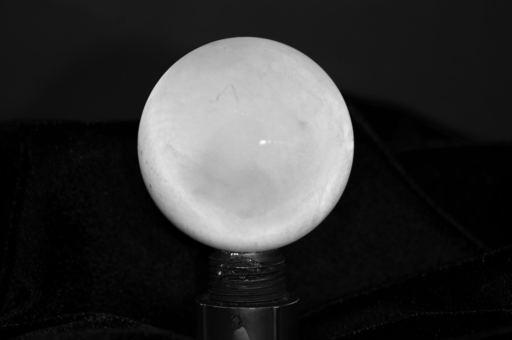
\includegraphics[width=\textwidth]{report_fig/gray_a}
        \end{subfigure}
        % second row
        \begin{subfigure}{0.3\textwidth}
                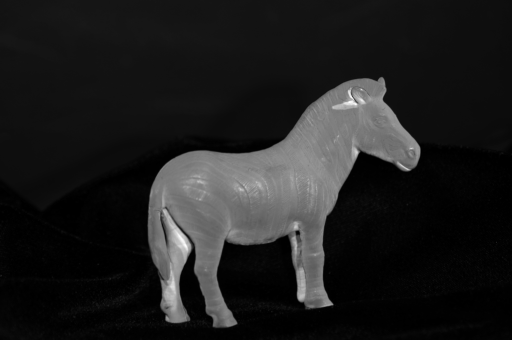
\includegraphics[width=\textwidth]{report_fig/horse_a}
        \end{subfigure}
        ~ 
        \begin{subfigure}{0.3\textwidth}
                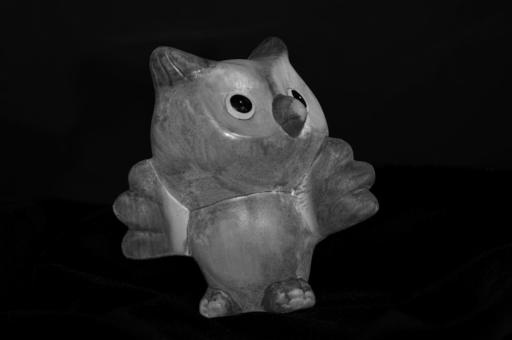
\includegraphics[width=\textwidth]{report_fig/owl_a}
        \end{subfigure}
        ~ 
        \begin{subfigure}{0.3\textwidth}
                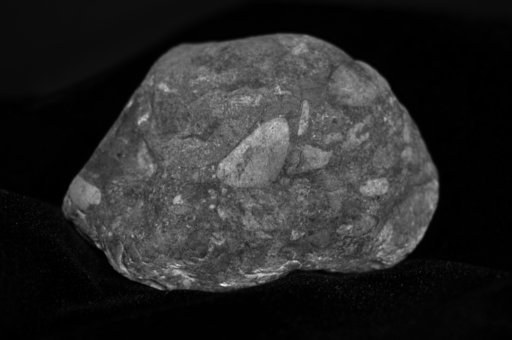
\includegraphics[width=\textwidth]{report_fig/rock_a}
        \end{subfigure}
        \caption{The grayscale albedo (luminance)}
        \label{fig:grayscale_albedo}
\end{figure}

\begin{figure}[h!]
        \centering
        \begin{subfigure}{0.3\textwidth}
                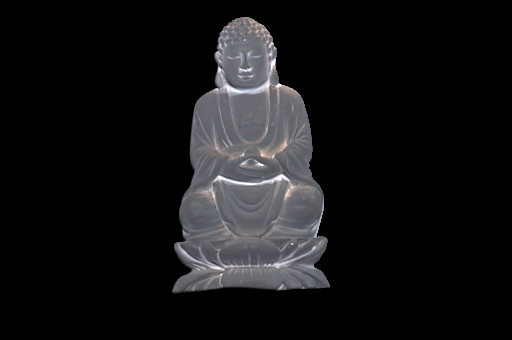
\includegraphics[width=\textwidth]{report_fig/buddha_ca}
        \end{subfigure}
        ~ 
        \begin{subfigure}{0.3\textwidth}
                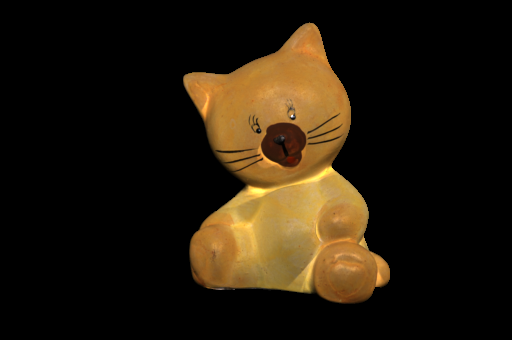
\includegraphics[width=\textwidth]{report_fig/cat_ca}
        \end{subfigure}
        ~ 
        \begin{subfigure}{0.3\textwidth}
                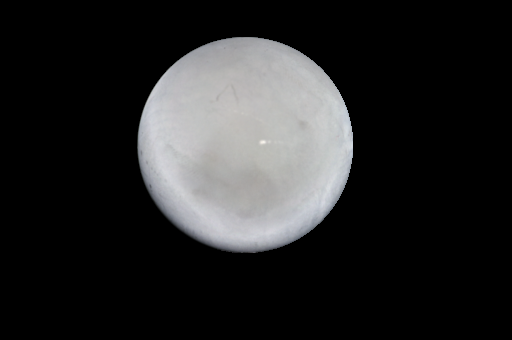
\includegraphics[width=\textwidth]{report_fig/gray_ca}
        \end{subfigure}
        % second row
        \begin{subfigure}{0.3\textwidth}
                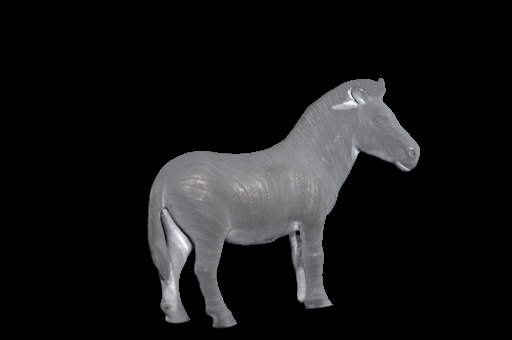
\includegraphics[width=\textwidth]{report_fig/horse_ca}
        \end{subfigure}
        ~ 
        \begin{subfigure}{0.3\textwidth}
                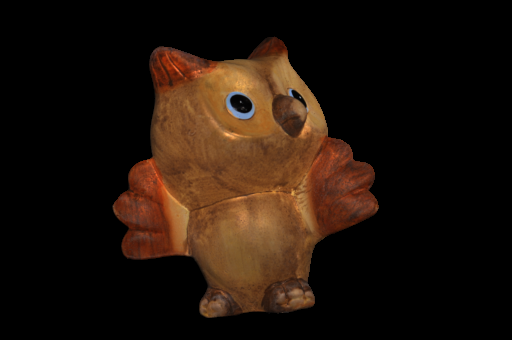
\includegraphics[width=\textwidth]{report_fig/owl_ca}
        \end{subfigure}
        ~ 
        \begin{subfigure}{0.3\textwidth}
                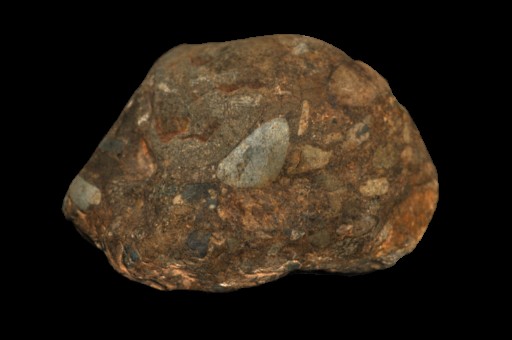
\includegraphics[width=\textwidth]{report_fig/rock_ca}
        \end{subfigure}
        \caption{The color albedo. The buddha, sphere and horse
        do in fact have a moreover gray albedo, so there is not too much
        of a difference to the grayscale albedo.}
        \label{fig:color_albedo}
\end{figure}

\subsection{Surface Fitting}

In this section you should:

\begin{itemize}
\item Describe the algorithm you used for calculating the depth map given the normals you calculated before.
\item Display the image of the depth map (in colour or grayscale) for each dataset, where higher intensity values indicate points closer to the camera.
\item Describe, in no more than a few paragraphs, your assessment of when the technique works well, and when there are failures. When the technique fails to produce nice results, please explain as best as you can what the likely causes of the problems are.
\end{itemize}















 \end{document}